\documentclass[12pt, aspectratio=169]{beamer} % aspectratio = either 43 or 169
\usepackage[utf8]{inputenc}
\usepackage{graphicx}
\usepackage[T1]{fontenc}
\graphicspath{ {./img/} }

\usetheme{Hannover}
\mode<presentation>

% title and author
\title{Presentación estudio tesis: Aplicación de metodologías de predicción de flujos de caja de los trabajadores autónomos españoles}
\author{Luis Palomero}
\date{2021-04-15}
% document
\begin{document}


\frame{\titlepage}


\begin{frame}{Overview}
\tableofcontents
\end{frame}

\section{Introducción y objetivos}

\begin{frame}{Introducción}
  \begin{itemize}
    \item Este es un proyecto de tesis asociado a un Doctorado Industrial, en colaboración con Declarando.
    \item Necesitamos poder realizar predicciones de los flujos de caja de los trabajadores autónomos de España.
    \item Es un proyecto realizado a media jornada. Su fecha de inicio ha sido finales de 2020.
  \end{itemize}

\end{frame}

\begin{frame}{Declarando}
  \begin{block}{Qué es Declarando}
    \begin{itemize}
    \item Startup española fundada en 2015.
    \item \textbf{Misión}: Ayudar a los 3 millones de autónomos españoles a ahorrar dinero y tiempo con sus impuestos.
    \item \textbf{Visión}: Automatizar el asesoramiento premium de los autónomos.
    \end{itemize}
  \end{block}
\end{frame}


\subsection{Contexto del proyecto}

\begin{frame}{¿Para qué queremos hacer estas predicciones?}
  \begin{block}{Para ofrecer producto}
    \begin{itemize}
    \item Esta investigación se plasmará en funcionalidad práctica que deberá realizar predicciones de forma automatizada y sin intervención directa.
    \end{itemize}
  \end{block}
  \begin{block}{Para ayudarles en la toma de decisiones}
    \begin{itemize}
    \item Predecir posibles descubiertos.
    \item Avisar si van a tener que tomar decisiones a nivel de impuestos.
    \end{itemize}
  \end{block}
  \begin{block}{Para que puedan acceder a financiación}
    \begin{itemize}
    \item Realizar informes de solvencia financiera.
    \end{itemize}
  \end{block}

\end{frame}



\section{Sobre los datos}
\begin{frame}{Overview}
\tableofcontents
\end{frame}


\begin{frame}{Datos actuales}
  
  Los usuarios son trabajadores autónomos españoles que tienen la obligación de presentar trimestralmente los ingresos y los gastos facturados.

  Cada usuario tiene (potencialmente) tres grandes tipos de datos:
  \begin{itemize}
  \item Perfil: Localización, edad, fecha de alta de autónomo, actividad/es, clientes, proveedores, etc.
  \item Ingresos y gastos.
  \item Cobros y pagos.    
  \end{itemize}

\end{frame}

\begin{frame}{Sobre los ingresos/gastos}
  \begin{itemize}
  \item Los usuarios presentan los modelos ante Hacienda a partir de estos datos.
  \item No terminan de ser datos fiables:
    \begin{itemize}
    \item Los cobros y pagos pueden ser de clientes/proveedores ``Varios''.
    \item Son datos insertados a mano. Puede haber olvidos.
    \end{itemize}
  \end{itemize}
\end{frame}

\begin{frame}{Sobre los cobros/pagos}
  \begin{itemize}
  \item Flujo directo de caja.
  \item Son datos \textit{más relevantes} que los de ingresos/gastos. 
  \item Son proporcionados directamente desde los datos de los a partir de una empresa intermedia, quienes también categorizan los movimientos.
  \item Está en fase de implantación, aún no hay información de muchos usuarios ni series temporales largas.
  \item Se va a ofrecer próximamente una tarjeta de débito que permita centralizar los pagos asociados a la actividad desde la misma.
  \end{itemize}
\end{frame}


\begin{frame}{Overview}
\tableofcontents
\end{frame}


\section{Trabajo realizado}


\begin{frame}

  Hemos dividido el trabajo en varias fases:
  \begin{itemize}
  \item \textbf{Fase 1}: Fase de \textit{warm-up}. Técnicas paramétricas univariadas.
  \item \textbf{Fases 2.1 y 2.2}: Exploración de técnicas no paramétricas y modelos multivariados.
  \item \textbf{Fases 3.1 y 3.2}: Incorporación de variables internas y externas a los usuarios en los modelos. Utilización de los registros diferentes usuarios para mejorar las predicciones.
  \end{itemize}

\end{frame}

\subsection{Plan de trabajo}

\begin{frame}{Fase 1: Warm-up}
  Esta primera fase es una toma de contacto con el problema.

  \begin{block}{Objetivo de esta fase}
    \begin{itemize}
    \item Tener una visión general del \textit{state of the art}.
    \item Hacer pruebas de concepto a nivel de definición de predicciones.
    \item Implementar un modelo de predicción paramétrico ya usable.
    \end{itemize}
  \end{block}

  \begin{figure}
    
\includegraphics[width=0.4\textwidth]{20210413_1_evaluation_shapshot.png}
    \label{fig:evalutaion}
  \end{figure}

\end{frame}

\begin{frame}{Fase 2: Exploración de técnicas no paramétricas y modelos multivariados}{Fase 2.1: Modelos no paramétricos}
  \begin{itemize}
  \item Explorar y comparar los modelos no paramétricos en caso del problema de la predicción de flujos de caja.
  \item Implementar los modelos más prometedores.
  \item Registrar y analizar resultados de la implementación. 
  \end{itemize}
\end{frame}

\begin{frame}{Fase 2: Exploración de técnicas no paramétricas y modelos multivariados}{Fase 2.2: Modelos multivariantes}

    \begin{itemize}
    \item Comparar las diferencias de \textit{performance} entre modelos univariados y multivariados a diferentes niveles (cobros/pagos, desglosando por clientes, etc.).
    \item Implementar los modelos más prometedores.
    \item Registrar y analizar resultados de la implementación. 
    \end{itemize}


\end{frame}


\begin{frame}{Fase 3: Exploraciones adicionales}

  \begin{block}{Fase 3.1: Incorporación de variables internas y exernas}
    \begin{itemize}
    \item Clasificación de usuarios según grupos.
    \item Estudio de la posibilidad de la predicción de posibles efectos externos en los flujos de caja.
    \end{itemize}
  \end{block}

  \begin{block}{Fase 3.2: \textit{Wisdom of the crowds}}
    \begin{itemize}
      \item{Estudio del efecto de los registros de datos del conjunto del resto de usuarios en la realización de las predicciones.}
    \end{itemize}
  \end{block}


\end{frame}

\subsection{Desarrollo ya realizado}

\begin{frame}{Desarrollo realizado}
  \begin{itemize}
  \item Barrido bibliográfico básico.
  \item Comparación con un \textit{benchmark}.
  \end{itemize}

\end{frame}

\begin{frame}{Barrido bibliográfico inicial}
  
  Se ha hecho un barrido bibliográfico muy breve centrado en el proceso de predicción de series temporales. Como ideas básicas se destaca que:
  \begin{itemize}
  \item La identificación de los problemas de \textit{clasificación de series}, \textit{imputación de valores faltantes} y la realización de \textit{previsiones} en si.
  \item Es un campo de aplicación tanto teórica como real.
  \item Las técnicas de \textit{machine learning} y \textit{deep learning} tienen mucho potencial.
  \end{itemize}
\end{frame}


\begin{frame}{Comparación con \textit{benchmark}}{Trabajo realizado}
  Se está finalizando una prueba de concepto en la que se replica una parte de los resultados del experimento del estudio del \textit{Parmezan'19}.
  \begin{block}{¿Qué se ha hecho?}
    \begin{itemize}
    \item Se implementan sobre 40 series sintéticas modelos paramétricos: Medias Móviles, Suavizado Exponencial, Modelo de Holt, Modelos de Holt-Winters, ARIMA/SARIMA. 
    \item Se realizan dos tipos de predicciones: aproximadas o actualizadas.
    \item Se implementa un método de validación que combina tres factores.
    \end{itemize}
  \end{block}
  Actualmente se ha realizado una primera iteración a falta de ser validada.

\end{frame}

\begin{frame}{Comparación con \textit{benchmark}}{Resultados preliminares}
  \begin{figure}
    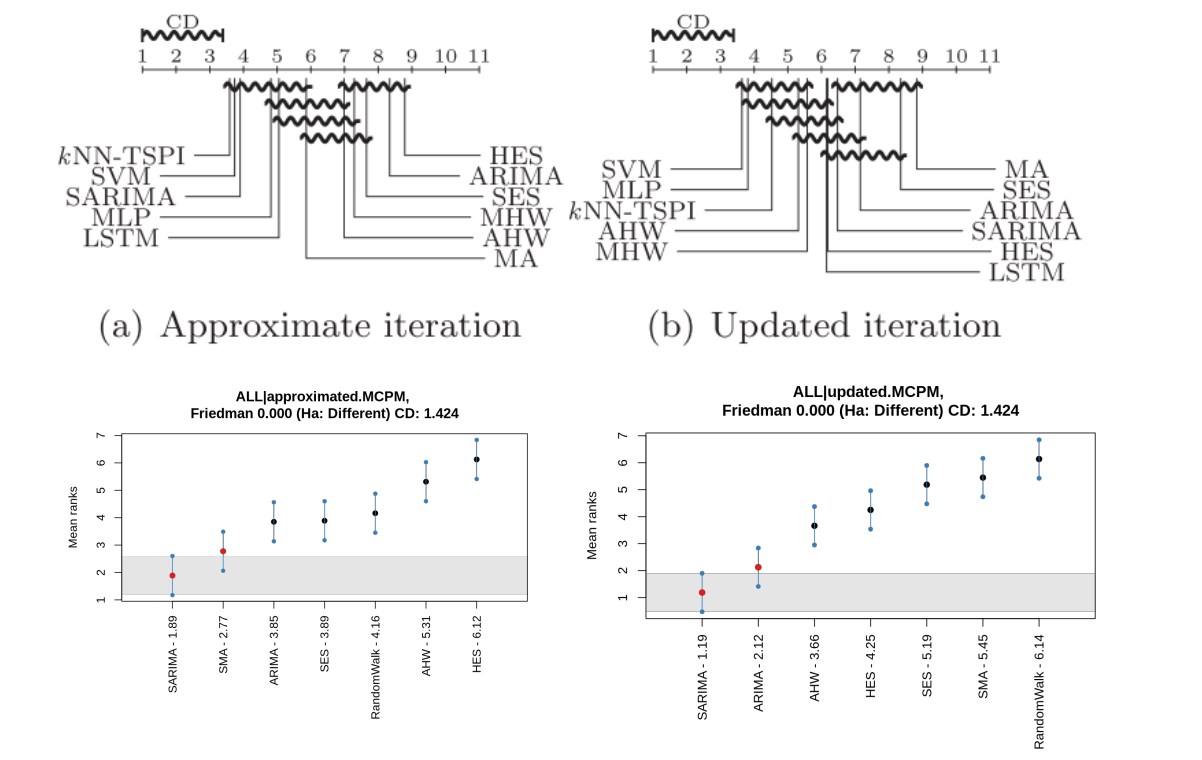
\includegraphics[width=0.8\textwidth]{20210413_2_resultados.png}
    \label{fig:resultados}
  \end{figure}
\end{frame}

\begin{frame}{Comparación con modelos ya realizados}{Idea de publicación}
  \textbf{Objetivo}: Combinar y profundizar el barrido con los resultados ya obtenidos para poder publicarlos.
  Estructura del un posible artículo inicial:
  \begin{itemize}
  \item \textbf{Introducción}: Presentación del problema de flujos de caja y las particularidades de las contabilidad.
  \item \textbf{Revisión bibliográfica}: Estudio del \textit{state of the art} y diferentes aproximaciones.
  \item \textbf{Análisis empíricos}: Réplica del estudio \textit{Parmezan'19} con sus datos y con los de Declarando.
  \item \textbf{Estudio de resultados}: Identificación de reglas de calidad para poder realizar predicciones con el mínimo número de muestras.
  \item \textbf{Resumen y discusión}: Descripción del trabajo realizado con métodos paramétricos y posibles \textit{next-steps}.
  \end{itemize}
\end{frame}



\section{Resumen}

\begin{frame}{Overview}
\tableofcontents
\end{frame}


\begin{frame}{Resumen}
  \begin{itemize}
  \item Necesitamos implementar algoritmos para poder predecir el flujo de caja de los trabajadores autónomos de forma automatizada.
  \item Hemos definido un plan de trabajo incremental, para poder ofrecer resultados publicables y utilizables lo antes posible.
  \item Estamos replicando un estudio ya publicado con resultados prometedores.
  \end{itemize}
\end{frame}


\begin{frame}{}
  \centering \Large
  \emph{Muchas gracias, ¿preguntas?}
\end{frame}


\end{document}
